\paragraph{}
    The in-situ data source is \textit{ORIENT HARBOR AT ORIENT NY}, but the remote data is worldwide with 4km resolution. Therefore, we limit our remote data to a polygon around the monitoring station.
    To reduce complexity, we choose this polygon to be a box with a latitudes range of $[40, 41.250] ^\circ N$ and a longitudes range of $[-73, -71]^\circ E$; this box encompasses an area of $25000\;km^2$ (refer to Fig 8).

    The remote data subset is spatial averaged to account for fluctuations inside the box.

\begin{figure}[H]
    \centering
    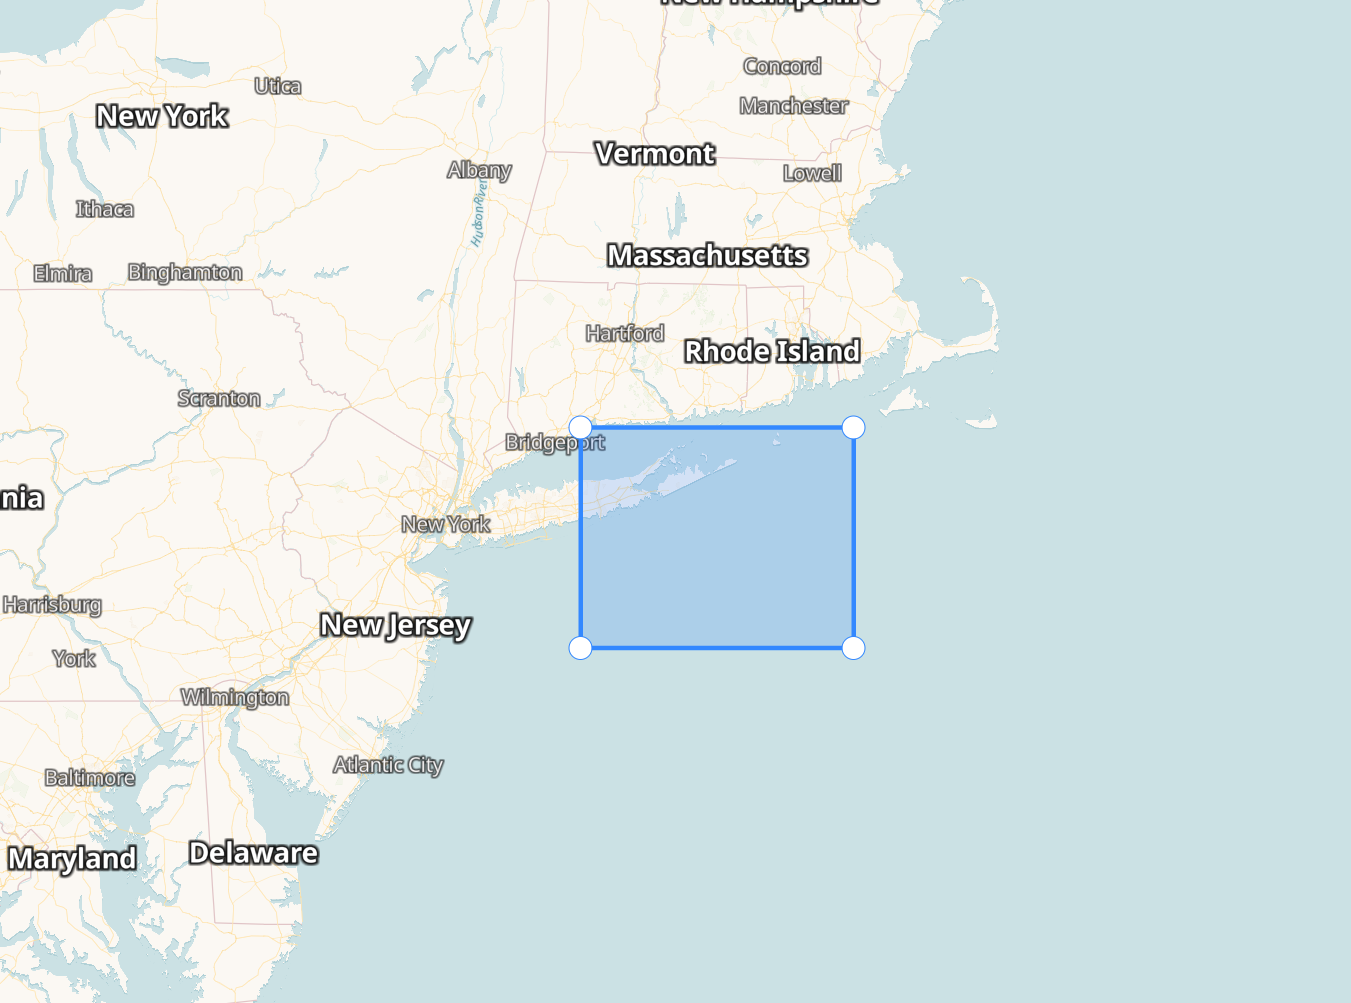
\includegraphics[scale=0.5]{figs/RSS_BOX.png}
    \caption{Subset for remote data}
\end{figure}


\paragraph*{}
    After gathering the data, we use the supervised machine learning algorithm called the \textbf{Multiple Linear Regression} to develop a relationship.
    \begin{equation}
        y = \beta_0 + \beta_1 x_1 + \beta_2 x_2 + \cdots + \beta_n x_n
    \end{equation}

    We have utilized pH, salinity, field temperature, remote temperature and specific conductance as our input parameters, so our equation will become
    \begin{equation}
        DO = \beta_0 + \beta_1 pH + \beta_2 (\text{salanity}) + \beta_3 (\text{field temperature}) + \beta_4 (\text{MODIS SST}) + \beta_5 (\text{specific conductance})
    \end{equation}

    We split our dataset into two sets, labeled for supervised learning and unlabled data for testsing with $0.8$ and $0.2$ ratio respectively.